\documentclass[main.tex]{subfiles}

\begin{document}
	
	\begingroup
	
	\renewcommand{\cleardoublepage}{}
	
	\renewcommand{\clearpage}{}
	
	\chapter{Grocery Task Overview}
	
	
	\chapterauthor{}
	
	\section{Goal}

	The goal which has to be achieved in the grocery task is to collect objects from a table and place them in a logical position in a shelf. The HSR has to autonomusly navigate the environment, it has to manipulate objects like doors and grocery items like chips, bananas etc. furthermore the HSR has to be able to lift items of the table and place them in the shelf where the final position of the moved object should either be grouped with similar objects (similarity is defined by size, color, shape and class) or open a new group apart from items which are not similar. The HSR has 5 minutes to achieve the given task. HIER FEHLT NOCH GENAUERE BESCHREIBUNG
	

	\section{Tasks}

		\begin{figure}	
			\centering
			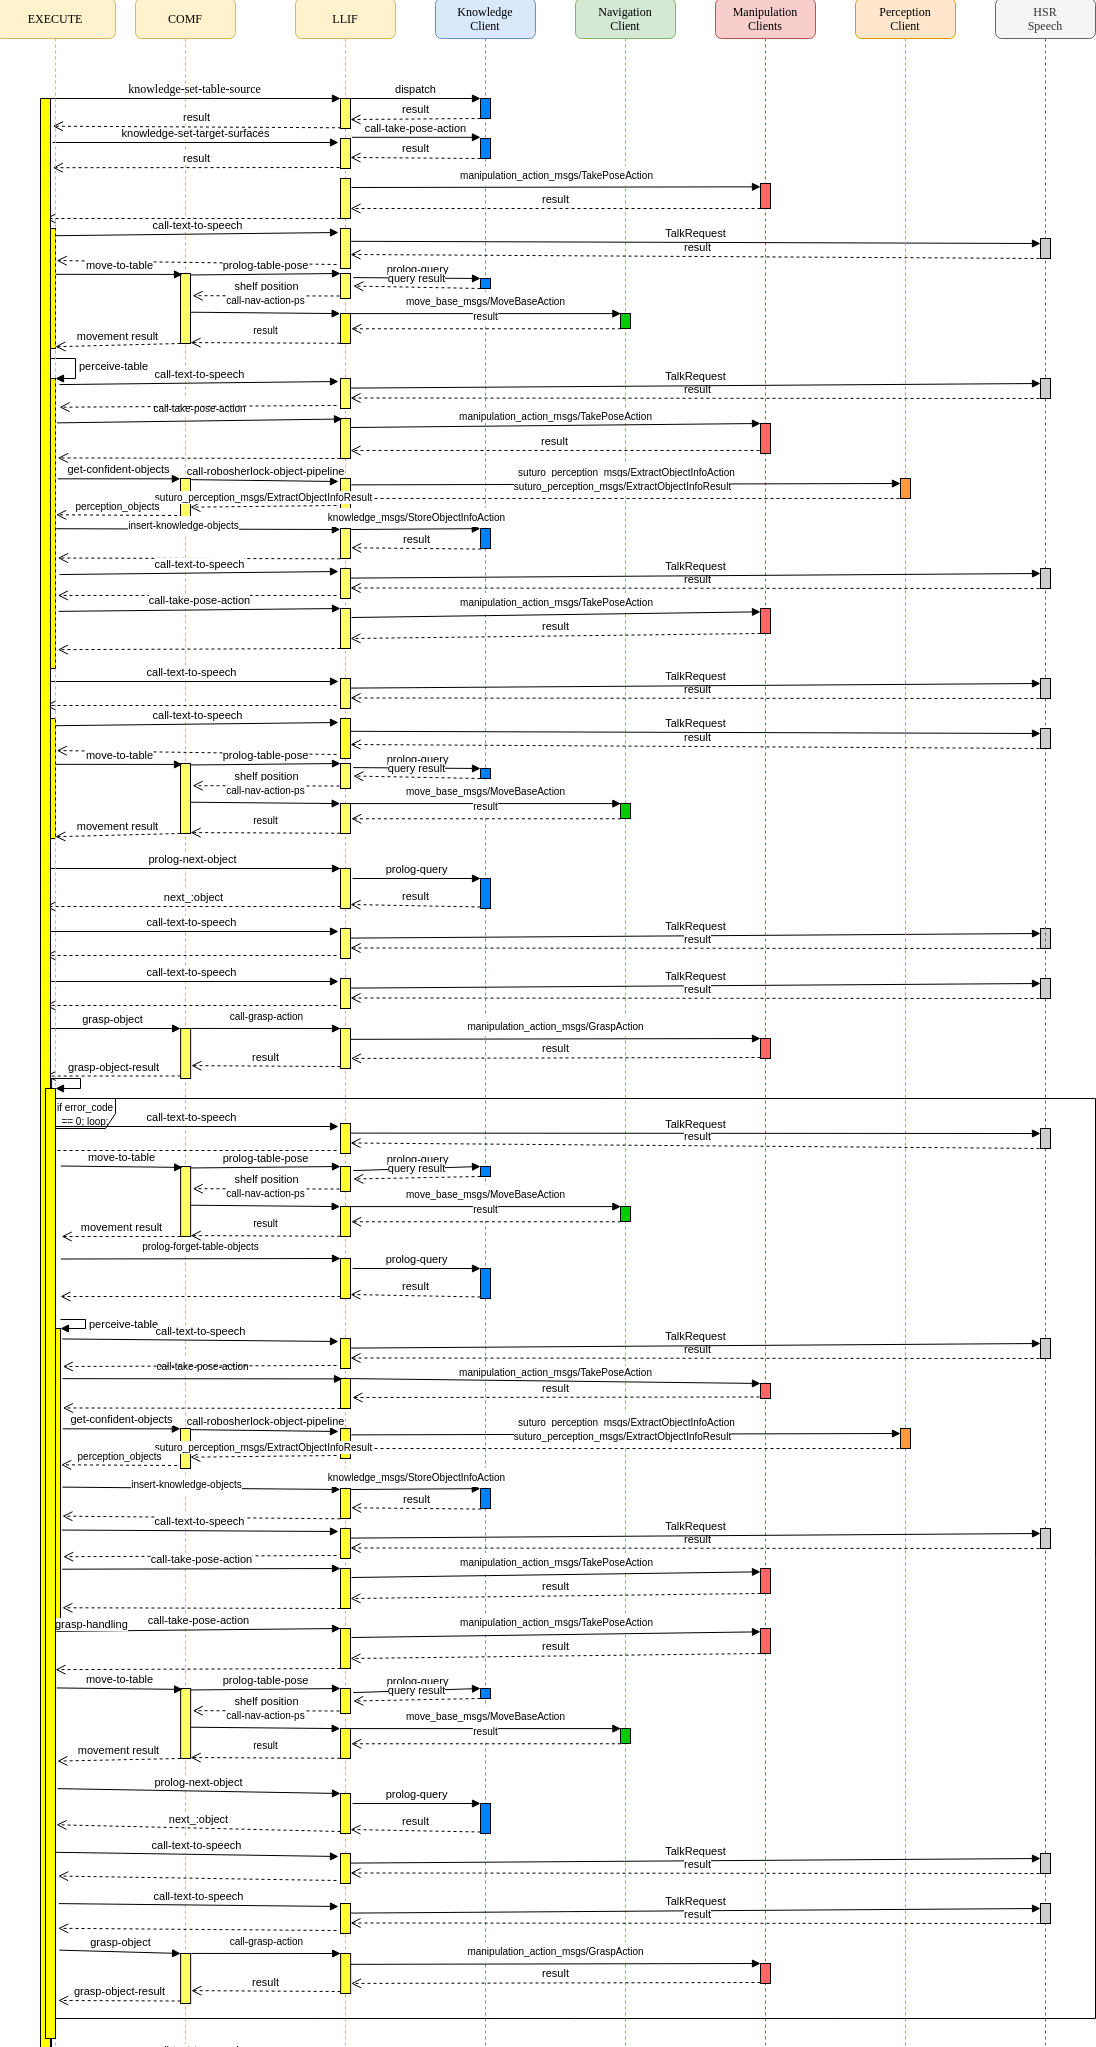
\includegraphics[width=0.85\textwidth]{pictures/diagramms/first-part-grocery-sequence.png}
			\caption{Sequence diagram of the complete run of the grocery storing task \textit{(explanations below)}}
			\label{grocery_seq_01}
		\end{figure}
		\begin{figure}	
			\centering
			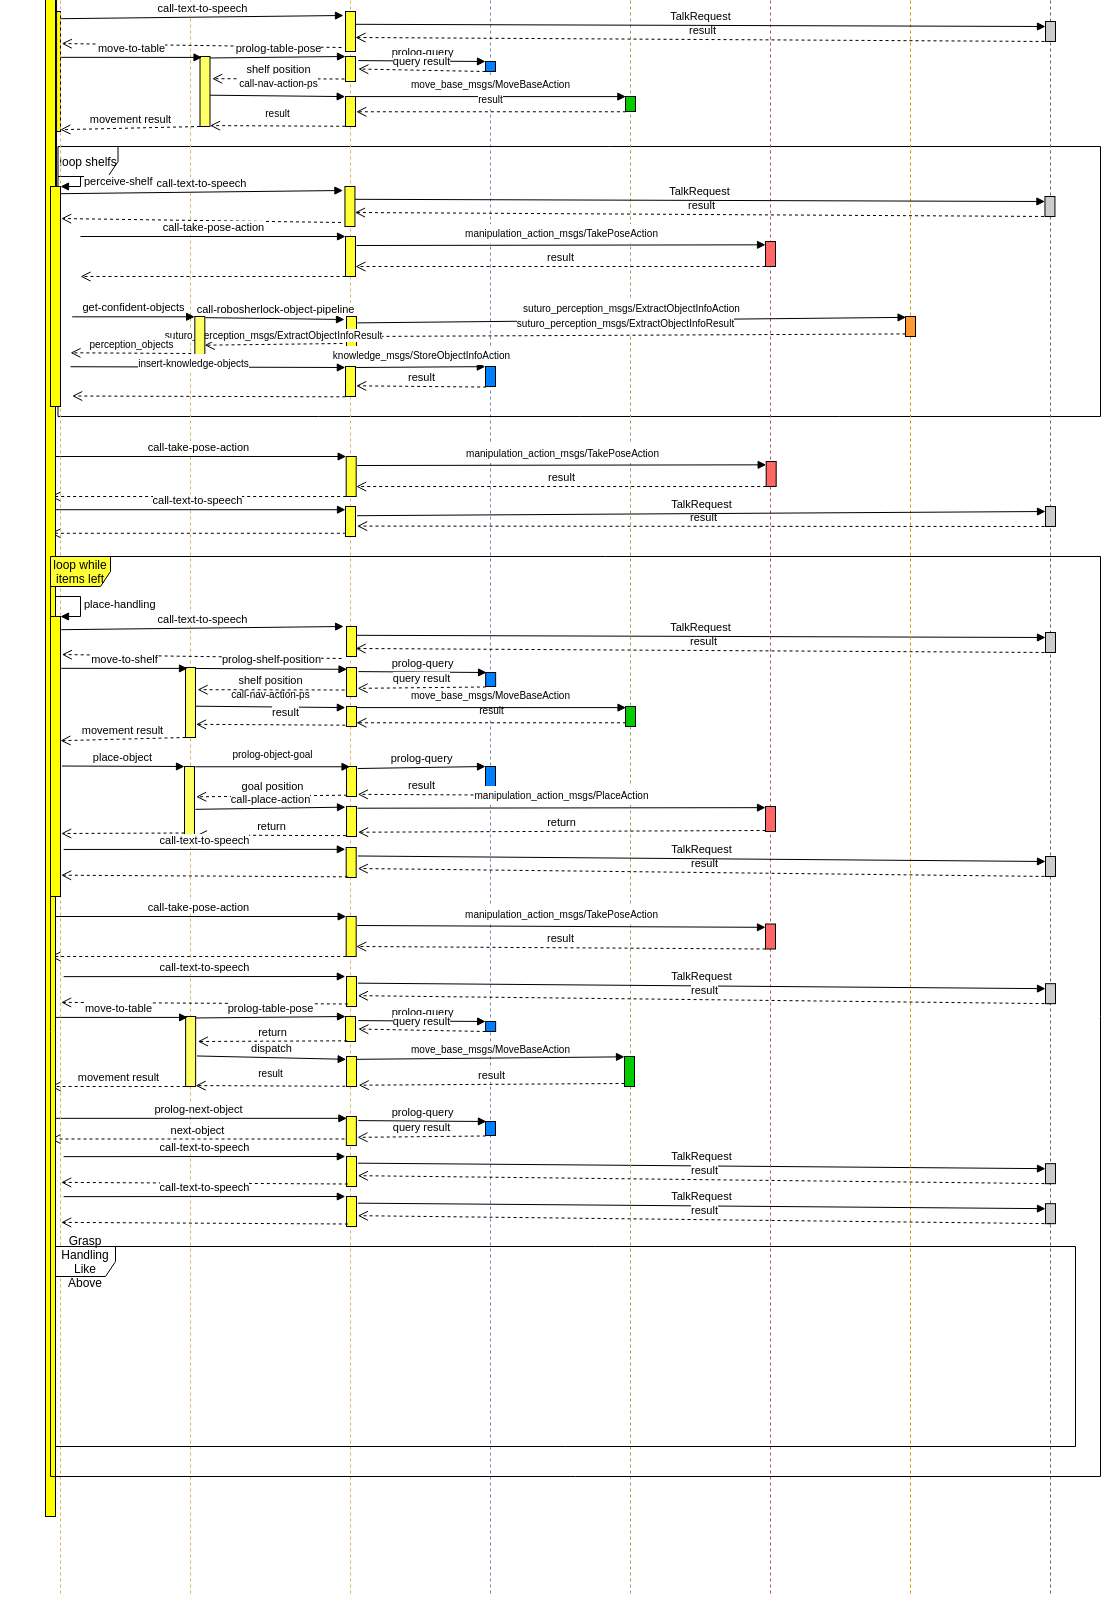
\includegraphics[width=0.85\textwidth]{pictures/diagramms/second-part-grocery-sequence.png}
			\caption{Sequence diagram of the complete run of the grocery storing task \textit{(explanations below)}}
			\label{grocery_seq_02}
		\end{figure}
	
	
<<<<<<< HEAD
		The sequence diagramm \ref{grocery_seq_01} and \ref{grocery_seq_02} does not depict when the actionservers are running it rather displays the time they are actively used.

	\section{Tasks}
	In the following subsections the execution and the procedure depicted in \ref{grocery_seq_01} and \ref{grocery_seq_02} will be explained in detail and include decisions made which let to the excact plan. Some more detail challanges will be explained aswell.
=======
		The sequence diagramm in figure \ref{grocery_seq_01} and \ref{grocery_seq_01} does not depict when the actionservers are running it rather displays the time they are actively used	
	
	In the following subsections the execution and the procedure depicted in figure \ref{grocery_seq_01} and \ref{grocery_seq_02} will be explained in detail and include decisions made which let to the excact plan. Some more detail challanges will be explained aswell.
>>>>>>> 4fbfa0fdfe5830e3faffcbcd07528105c1d616bf

	At first the definition of the task is set in knowledge: We want to find objects on all the tables, so all the table surfaces are set as \texttt{source} and we want to place the found objects in shelves, so all the shelves are set as \texttt{target}. This procedure enables Knowledge, to genetically work over \texttt{source} and \texttt{target} surfaces regardless of what they actually are.
	
	% Manipulation: take pose action
	
	% NLP: Talk Request
	
	% Knowledge: get ttable-poses
	
	% Navigation: moveBaseAction
	
	% NLP: Talk Request
	
	% Manipulation: TakePoseAction
	
	% Perception: Percieve and return data
	
	% Knowledge: Store Data
	
	% NLP: Talk Request
	
	% Manipulation: Take pose
	
	% 2x NLP: Talk
	
	% Knowledge: get shelf poses
	
	% Manipulation: move to table
	
	% 

	\subsection{perceive table sequence}
	At the beginning we planned to scan the shelf first but during testing we found out that it will take less time to scan the shelf with the first object already in hand so the HSR scans the table for this perception, planning and knowledge had to do ...........

	\subsection{grasp preparation sequence}
	\subsection{handle grasp failure sequence}
	\subsection{travel sequence}
	Maybe too redundant....
	\subsection{loop shelfes sequence}
	\subsection{main loop sequence}
	
	\section{Conclusion}

	We achieved the task blash blash blash ...
	
	
	\endgroup
	
\end{document}
